\chapter{Introduction}
% Introduction section
%  1. Introduction.
%  2. Background and setting. 
%  3. Identification of problem
%  4. Purpose Statement. 
%  5. Objectives or research questions
%  6. Assumptions. Limitations. Definition of terms
%  7. Significance of the study.

% Introduction section (from unsw.edu.au)
% Move A: establish your territory (say what the topic is about)
%   1.  state the general topic and give some background
%   2.  provide a review of the literature related to the topic
%   3.  define the terms and scope of the topic
Optimization plays an important part in our everyday life, science development, and product design.
What transportation should you choose to get fast from A to B? What songs should
land on your playlist? and what is the optimal bridge construction? In general, optimization is the
art of choosing the best decision. Often we can quantify how good a decision is: A bus takes 20 min,
a car takes 15 min to go from A to B, How would you rate the song?
This bridge construction costs 10 million. If it is possible to come up with a quantification of how good
a decision is in terms of a real number, then we can define is a \textit{mathematical optimization problem}: 
$$\min_{x\in \mathcal{X}} f(x)$$ where the functional $f: \mathcal{X} \rightarrow \mathbb{R}$ is
called the objective function and $\mathcal{X}$ is the set of possible decisions (or decisions you consider).
The optimization problem is now in the domain of cold numbers and here many algorithms have been developed
to find the minimum of the function $f(\cdot)$. Note that we throughout this thesis refer to
optimization as minimizing a cost function - this is equivalent to maximizing the negated function
$\max_{x\in \mathcal{X}} f(x) = \min_{x\in \mathcal{X}} -f(x)$.  

Evaluation of the objective function can be cheap e.g. if it just requires
summing and multiplying numbers or highly expensive if it involves human rating or large simulation
and physical experiments. Bayesian optimization is a preferred <ref> framework for optimization of
the expensive objective functions. And is also referred to as \textit{sample efficient}
optimization.

Bayesian optimization is a probabilistic surrogate-based optimization methodology: Assuming some samples from a
highly expensive objective a cheap (surrogate) function is used to fit the samples. The next sample
is found by minimizing the surrogate and the process is repeated. Bayesian optimization seeks to
enhance this procedure with probability theory, where the surrogate function becomes a probabilistic
regression model. The most common choice is a Gaussian Process, as it encapsulates the uncertainty very well,
but also because its inference procedure (computing answers to probability queries like $p(y|x)$) is exact.

% Move B: establish a niche (show why there needs to be further research on your topic)
%   4.  outline the current situation
%   5.  evaluate the current situation (advantages/ disadvantages) and identify the gap

\section{Weakness of GPs}
Using GP with isotropic kernel function, have continous sample paths, 
which might be undesired . 


Even though GP has proven good for many cases, there will be problems where the assumptions do not hold. 
The assumptions of a GP are essential that the objective function can be described as a GP.
The nature of a GP is highly dependent on the choice of its kernel and the parameters chosen in that kernel. 
Another reason for the popularity of the GP is the closed-form inference and giving a closed-form of the 
expected improvement acquisition function. 

$$p(y|x, \mathcal{D}) = GP(f(x)|\mu(x), \kappa(x,x)) \implies x_{next} = \arg\max_x \sigma_x [u\Phi(u)+ \phi(u)]$$


% Move C: introduce the current research (make hypotheses; state the research questions)
%   6.  identify the importance of the proposed research
%   7.  state the research problem/ questions
%   8.  state the research aims and/or research objectives
%   9.  state the hypotheses
%   10. outline the order of information in the thesis
%   11. outline the methodology

\section{No free lunch and surrogate reseach}

<No free lunch theorem for optimization>, establish some questions on why there is no best method.
And a burning research problem is if it is possible to use a different surrogate model than the GP. 
And whether or not they in general performs better? What assumptions underlie the problem. 
The assumption for GP regression is that the objective function follows a Gaussian process, whereas
we assume it follows a random forest or neural network. These are assumptions that yields, consideration:
Is this a good assumption? Bayesian NNs are very expressive. 

Bayesian multivariate adaptive
regression splines (BMARS)30,31 and Bayesian additive regression
trees (BART)32 a
shows superior when f, requires more flexible model. 

surrogates: 
\begin{itemize}
    \item GP
    \item BNN
    \item Random forest
    \item SPN
    \item Kernel estimator
\end{itemize}

Within Bayesian surrogate model, there has been research on using random forest or Bayesian neural 
networks. The PhD thesis "Sample-efficient Optimization Using Neural Networks" from 2020 \cite{PhDthesis}
showcases empirically that using Bayesian neural networks as surrogate models performed better,
or at least comparable to GPs on a wide number of problems. The performance difference was more
clear for high-dimensional problems. 

While most alternative method are investigated due to the expensive inference time for GPs, 
this thesis investigates alternative surrogates as a method of 

Another regression model not seen much in the literature is Gaussian mixture regression, which
is modeling the joint distribution between x and y, and using the conditional distribution $p(y|x)$
as the regression model, which is provided exactly. 

Research problem/question:
\begin{itemize}
    \item Which type of optimization problem is a GP not a good choice?
\end{itemize}

\begin{figure}[H]%
    \centering
    {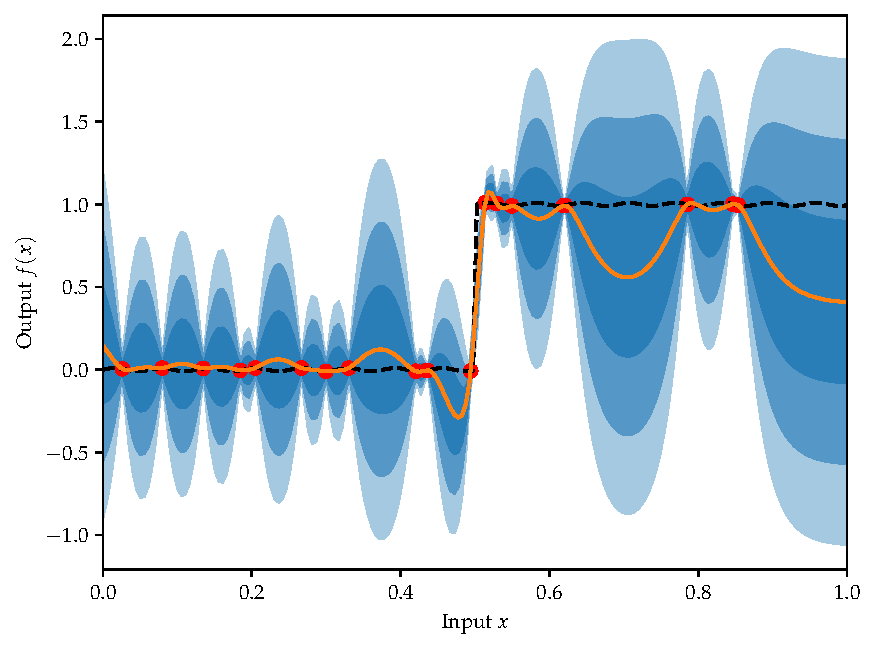
\includegraphics[width=0.46\textwidth]{Pictures/GP_vs_BNN1.pdf} }%
    \qquad
   {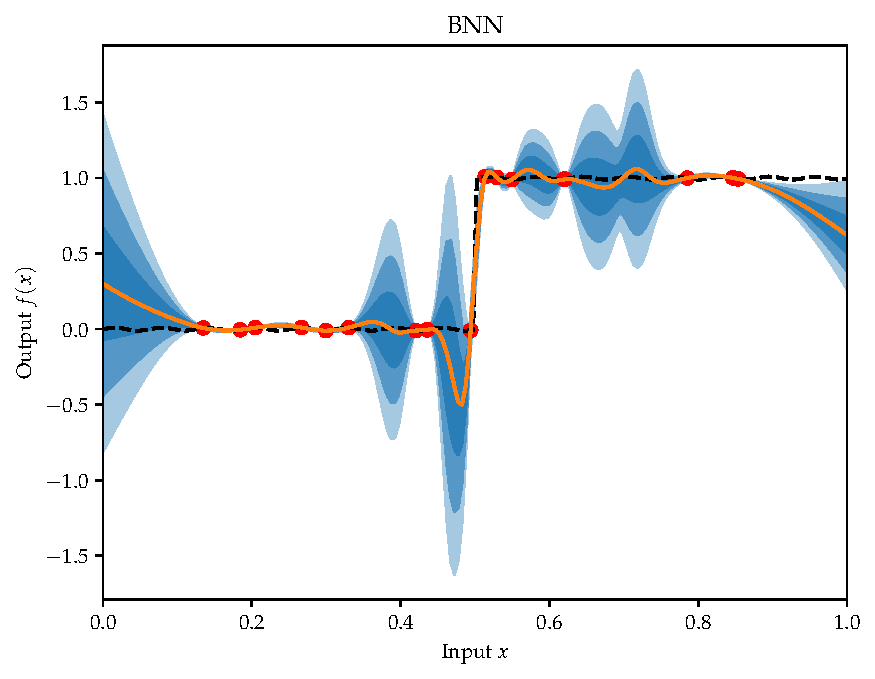
\includegraphics[width=0.46\textwidth]{Pictures/GP_vs_BNN2.pdf} }%
    \caption{Example where The discontinuerity makes the GP overreact to all other 
    uncertainties}%
    \label{fig:example}%
\end{figure}


Research aims:
As a new model Sum product networks has become a promissing method. Shown to be the most 
general probabilistic model that allows for exact inference! <ref>. It has relation to 
neural networks (but with the limit of not being too deep) and Bayesian networks, and provides
a framework for learning and inference in deep probabilistic models. As nice as it sounds
the project will investigate what SPNs are and how it can be used as a surrogate models. 

As we will see later SPNs are just exponentially large mixture models, and therefore 
it is interesting to investigate Kernel estimators.

state the hypotheses
\begin{itemize}
    \item Will an SPN work as a surrogate model?
    \item We can find problems where GPs fails to establish good predictions. 
    \item BNN might work as well as GPs
\end{itemize}

%   10. outline the order of information in the thesis
%   11. outline the methodology


\section{Old intro}
%<What is optimization>
Optimization plays an important part in our everyday life, science development, and product design.
What different transportation should you choose to get fast from A to B, what songs should
land on your playlist, and what is the optimal bridge construction. Mathematical optimization problems 
are all problems in the form, 
$$\min_{x\in \mathcal{X}} f(x)$$ where $f: \mathcal{X} \rightarrow \mathcal{R}$ is a functional. I.e
if it is possible to set up an objective function. e.g. what is the cost of the bridge given a
specific design, or how pleasant you think some music, and some constraints such that you keep in
the domain of interest. Evaluation of the objective function can be cheap e.g. if it just requires
summing and multiplying numbers or highly expensive if it involves human rating or large simulation
and physical experiments. Bayesian optimization is a preferred <ref> framework for optimization of
the expensive objective functions. And is also referred to as \textit{sample efficient}
optimization. 
%<Why Bayesian optimization?>

Bayesian optimization is a probabilistic surrogate-based optimization: Assuming some samples from a
highly expensive objective a cheap (surrogate) function is used to fit the samples. The next sample
is found by minimizing the surrogate and the process is repeated. Bayesian optimization seeks to
enhance this procedure with probability theory, where the surrogate function becomes a probabilistic
regression model. The most common choice is a Gaussian Process, as it encapsulates the uncertainty very well,
but also because its inference procedure (computing answers to probability queries like $p(y|x)$) is exact.

Even though GP has proven good for many cases, there will be problems where the assumptions do not hold. 
The assumptions of a GP are essential that the objective function can be described as a GP.
The nature of a GP is highly dependent on the choice of its kernel and the parameters chosen in that kernel. 
Another reason for the popularity of the GP is the closed-form inference and giving a closed-form of the 
expected improvement aqurisition function. 

The PhD thesis "Sample-efficient Optimization Using Neural Networks" from 2020 \cite{PhDthesis}
showcases empirically that using Bayesian neural networks as surrogate models performed better,
or at least comparable to GPs on a wide number of problems. The performance difference was more
clear for high-dimensional problems. 

This master thesis project will investigate surrogate models alternative to Gaussian processes in
Bayesian optimization. Firstly by examining what types of problems a GP surrogate is not a good
choice for and where Bayesian neural nets (BNN) surrogates can have an advantage (inspiration found in
this 2020 thesis [1]). Secondly by looking at sum-product networks (SPN) as novel surrogate models.
An SPN is - similarly to a BNN - a deep probabilistic model and still expressive but with tractable
inference, which potentially could lead to advantages over BNNs. 

%#<Short overview of types of surrogate models>

<Make a figure of how the parts are all connected>

\section{notation}
Throughout this thesis we will be using Bayesian notation, i.e. $p(x) := P(X=x)$ is 
the probability density function of the random variable $X$ evaluated in $x$. 
and $p(y|x) := P(Y=y|X=x)$ or $p(y|x) := P(Y|X=x)$.

And writing $p(y^2|x)$ means $P(Y^2=y^2|X=x)$ and \textbf{not} $P(Y=y^2|X=x)$

\section{related work}
This thesis is 
<BAHAMIANN>

<DNGO>
Focus on the inference time of GP scales cubic, which is not appropriate for
parallel BayesOpt. 
Experiments on 6dim Hartmann function. 

<Arayns paper.>
Conclusions..!?

Already developed alternative surrogate models has been found in the litterateur. The last presented
surrogate model, SPN, is to our knowledge not in any published work. More models might still be
added to the list. 

\subsubsection*{DNGO}
Deep Networks for Global Optimization (DNGO) is presented in the paper 2015 paper "Scalable Bayesian
Optimization Using Deep Neural Networks"\cite{snoek2015scalable}. The surrogate model is a neural
network, where only the last layer is probabilistic, this leads to Bayesian regression and very fast
inference.  

\subsubsection*{BOHAMIANN}
\textbf{B}ayesian \textbf{O}ptimization with \textbf{Hami}ltonian Monte Carlo \textbf{A}rtificial
\textbf{N}eural \textbf{N}etworks (BOHAMIANN) is presented in the 2016 paper "Bayesian Optimization
with Robust Bayesian Neural Networks"\cite{NIPS2016_a96d3afe}. This is a fully Bayesian Neural
Network trained using adaptive Hamiltonian MCMC. 